% !TEX root = thesis-thomas-tiotto.tex

\section{Methods}
\subsection{Libraries}
\subsubsection{pomegranate}
Pomegranate (\cite{pomegranate}) is an open-source probabilistic models package for python.
Its core philosophy is that every probabilistic model, from Hidden Markov to Bayesian Network, can be seen as a probability distribution and, as such, can be flexibly composed into hierarchical mixture models (\cite{Schreiber2017}).
The package implements:
\begin{itemize}
	\item Probability Distributions
	\item General Mixture Models
	\item Hidden Markov Models
	\item Bayes Classifiers and Na{\"i}ve Bayes
	\item Markov Chains
	\item \textbf{Bayesian Networks}
	\item Factor Graphs
\end{itemize} 

This package was chosen among others for its good implementation of Bayesian Networks, its clear API and its performance.
The package is written in cython and natively supports multi-core parallelism and out-of-core learning.
Network structure learning from data, described in \ref{subsec:bnstructurelearning}, appears to be particularly efficient, thanks to the implementation of prior knowledge into the graph selection process as described by \cite{schreiber_noble_2017}.
The claim of this novel selection process is that it possesses the speed of a heuristic approach while yielding a far better quality estimate.

pomegranate currently only supports Discrete Bayesian Networks so the random variable of each node must have a categorical distribution.

\textit{Structure learning} from data is achieved using the \texttt{from\_samples} method of the \texttt{BayesianNetwork} class, with the default algorithm being the novel one described by \cite{schreiber_noble_2017}.
The \textit{probability} of a sample is calculated using the \texttt{probability} function of an object of \texttt{BayesianNetwork} type; the \texttt{predict\_proba} function is used to return the probability of each variable in the model given some evidence.
\textit{Predictions} (described in detail in Sec. \ref{subsec:bnupdating}) are run by passing to the \texttt{predict} function of an object a matrix with \texttt{None} as placeholders for missing values .
\textit{Fitting} is done thought the \texttt{fit} function that uses MLE estimates to update each node's distribution in the model based on the input data.

A \texttt{BayesianNetwork} object can also be displayed graphically by calling its \texttt{plot} function.
The output is a DOT file that is generated using the PyGraphviz package (\cite{pygraphviz}), that is a python interface to the famous Graphviz (\cite{graphviz}) graph visualisation software.
An example of such an output is shown in Fig. \ref{fig:pomegranate_graph_example}.

\begin{figure}[htbp]
\centerline{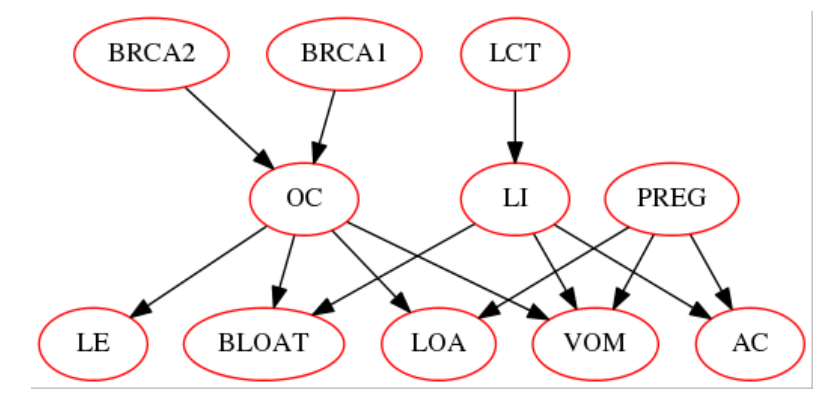
\includegraphics[width=\columnwidth]{methodology/images/pomegranate_example}}
\caption{Example output of \texttt{plot} (\cite{pomegranatetutorial}) }
\label{fig:pomegranate_graph_example}
\end{figure}

\subsubsection{pandas}
\subsubsection{scikit-learn}
\subsubsection{numpy}
\subsubsection{networkx}
\subsection{Algorithms}
\subsubsection{d-separation}
\subsubsection{MPE}